% !TeX encoding = UTF-8
% !TeX spellcheck = en_US

\documentclass[ 
% amsmath=
% amsthm=
% array=
% calc
% enumerate=
% extsizes
% geometry
% hyperref
xcolor={usenames,dvipsnames,svgnames,tablem} 
%,bigger
,handout
]{beamer}
% automatically loaded: xcolor, amsmath, amsthm, calc, geometry, hyperref, extsizes

% \input{HEADER/HEADER}

% !TeX root = ../m3Headout.tex
% !TeX encoding = UTF-8
% !TeX spellcheck = en_US

%% ==============================================================
%% ### BEAMER ###

\usetheme[]{CambridgeUS}	
\usecolortheme{seagull}			% seahorse, fly, dolphin, dove, beetle, seagull ...
\useinnertheme{circles}			% tree, smoothtree, infolines, smoothbars	
\usefonttheme{professionalfonts} 	% professionalfonts serif structurebold structureitalicserif structuresmallcapsserif
	
\beamertemplatenavigationsymbolsempty

%% ==============================================================
%% ### "PACKAGES" ###

% BY BEAMER: xcolor, amsmath, amsthm, calc, geometry, hyperref, extsizes

\usepackage{calc}

\usepackage[utf8x]{inputenc} 		% Eingabekodierung	
\usepackage[english]{babel}	
\usepackage[T1]{fontenc}	 		% Ausgabekodierung (PDF)
%\usepackage[
	%usenames,
	%dvipsnames,
	%svgnames,
	%table]{xcolor} 				% BEAMER, Farben
%\usepackage{amsmath}				% BEAMTER
%\usepackage{amsthm}				% BEAMTER
\usepackage{amssymb}				% \ngtpreq

\usepackage{proof} 					%\infer, \deduce
%\usepackage{marvosym}				% \Lightning

%\usepackage{soul}					% \so\caps\ul\st\hl
%\usepackage[normalem]{ulem} 		% \uline\uuline\sout\xout\uwave
%\usepackage{transparent}
\usepackage{listings} 			% are there some issues ?
%\usepackage{multirow}
%\usepackage{pdfpages}

%\usepackage[weather]{ifsym} 	% does not work with tex writer
%\let\Sun\relax 				% defined in marvosym too
%\let\Lightning\relax 			% defined in marvosym too

%\usepackage{ulsy}				% \blitza \blitzb ... \blitze (does not exist anymore? just not included?)

\usepackage{tabularx}

\usepackage{pifont} 			% dingbats

% setup listing

\lstdefinelanguage{smtlib}{
	comment={[l];},
	keywords={assert,xor, or, and},
	otherkeywords={declare-fun, set-logic},
	emph={Int,QF_LIA},
}

\lstset {
	backgroundcolor=\color{white},     	% choose the background color; you must add \usepackage{color} or \usepackage{xcolor}
	basicstyle=\ttfamily\footnotesize, 	% the size of the fonts that are used for the code
	breakatwhitespace=false,         	% sets if automatic breaks should only happen at whitespace
	breaklines=true,                 	% sets automatic line breaking
	captionpos=b,                    	% sets the caption-position to bottom
	commentstyle=\color{gray},    		% comment style
	deletekeywords={...},            	% if you want to delete keywords from the given language
	emphstyle=\color{orange},
	escapeinside={\%*}{*)},         % if you want to add LaTeX within your code
	extendedchars=true,             % lets you use non-ASCII characters; for 8-bits encodings only, does not work with UTF-8
	frame=none,		% frame=single, % adds a frame around the code
	keepspaces=true,                % keeps spaces in text, useful for keeping indentation of code (possibly needs columns=flexible)
	keywordstyle=\color{blue},      % keyword style
	% language=smtlib,	%Octave,    % the language of the code
	% literate={;},
	% otherkeywords={declare-fun,set-logic,assert,xor,or,and},            % if you want to add more keywords to the set
	%morecomment=[l]{;}				% line comment
	numbers=left,                   % where to put the line-numbers; possible values are (none, left, right)
	numbersep=5pt,                  % how far the line-numbers are from the code
	numberstyle=\tiny\color{gray}, 	% the style that is used for the line-numbers
	rulecolor=\color{black},        % if not set, the frame-color may be changed on line-breaks within not-black text (e.g. comments (green here))
	showspaces=false,               % show spaces everywhere adding particular underscores; it overrides 'showstringspaces'
	showstringspaces=false,         % underline spaces within strings only
	showtabs=false,                 % show tabs within strings adding particular underscores
	stepnumber=2,                   % the step between two line-numbers. If it's 1, each line will be numbered
	stringstyle=\color{orange},     % string literal style
	tabsize=2,	                   	% sets default tabsize to 2 spaces
	title=\lstname                  % show the filename of files included with \lstinputlisting; also try caption instead of title
}

\input{../HEADER/Colors}
% !TeX encoding = UTF-8

% shortens the definition by cases
\newcommand{\DEFINE}[3][=]{{
		\begin{gather*}
		#2 #1 \left \{
				\begin{array}{ll}
					#3
				\end{array}
		\right.
		\end{gather*}
	}}


% accepts greek as input
\newcommand{\textgreek}[1]{\begingroup\fontencoding{LGR}\selectfont#1\endgroup}

\newcommand{\tikzmark}[1]{\tikz[overlay,remember picture] \node (#1) {};}



\documentclass[]{clseminar}

    \documentclass[]{clseminar}

    \documentclass[]{clseminar}

    \input{../PREAMBLE/Symbols}
    
    \begin{document}
    
    \author{Alexander Maringele}
    \title{Symbols}
    \abstract{The quick brown fox jumps over the lazy dog.
    Why?}
    
    \maketitle

    \newcommand{\demo}[1]{$#1$}

    \begin{itemize}
        \item \verb+\myem+ \myem The quick brown fox jumps over the lazy dog
        \item 
        \demo{\disjointunion},,
        \verb+\disjointunion+ 
        $\disjointunion$, 
        \verb+\false+ 
        $\false$,
        \verb+\lbic+ 
        $\lbic$,  
        \verb+\limp+ 
        $\limp$,  
        \verb+\succG\succL\succC+
        $\succG$,   
        \verb+\succG\succL\succC+
        $\succL$,   
        \verb+\succG\succL\succC+
        $\succC$, 
        \verb+\true+ $\true$

    \end{itemize}



    
        
    \end{document}
    
    \begin{document}
    
    \author{Alexander Maringele}
    \title{Symbols}
    \abstract{The quick brown fox jumps over the lazy dog.
    Why?}
    
    \maketitle

    \newcommand{\demo}[1]{$#1$}

    \begin{itemize}
        \item \verb+\myem+ \myem The quick brown fox jumps over the lazy dog
        \item 
        \demo{\disjointunion},,
        \verb+\disjointunion+ 
        $\disjointunion$, 
        \verb+\false+ 
        $\false$,
        \verb+\lbic+ 
        $\lbic$,  
        \verb+\limp+ 
        $\limp$,  
        \verb+\succG\succL\succC+
        $\succG$,   
        \verb+\succG\succL\succC+
        $\succL$,   
        \verb+\succG\succL\succC+
        $\succC$, 
        \verb+\true+ $\true$

    \end{itemize}



    
        
    \end{document}
    
    \begin{document}
    
    \author{Alexander Maringele}
    \title{Symbols}
    \abstract{The quick brown fox jumps over the lazy dog.
    Why?}
    
    \maketitle

    \newcommand{\demo}[1]{$#1$}

    \begin{itemize}
        \item \verb+\myem+ \myem The quick brown fox jumps over the lazy dog
        \item 
        \demo{\disjointunion},,
        \verb+\disjointunion+ 
        $\disjointunion$, 
        \verb+\false+ 
        $\false$,
        \verb+\lbic+ 
        $\lbic$,  
        \verb+\limp+ 
        $\limp$,  
        \verb+\succG\succL\succC+
        $\succG$,   
        \verb+\succG\succL\succC+
        $\succL$,   
        \verb+\succG\succL\succC+
        $\succC$, 
        \verb+\true+ $\true$

    \end{itemize}



    
        
    \end{document}
\input{../HEADER/Drawing}


\renewcommand{\ORIGIN}{}
\providecommand{\PAUSE}{}

\author{Alexander Maringele}
\title{flea}
\subtitle{system description}
\date{September 2016 -- Obergurgl}

\begin{document}

% ==============================================================
\frame{\maketitle}

% ==============================================================
\frame{
	\frametitle{Refutation}
	% !TeX spellcheck = en_US
% !TeX encoding = UTF-8

\begin{tikzpicture}[scale = 1, transform shape, draw=black, fill=black, thick, sloped]

	\draw[myarrow, ultra thick] (0,0) -- 
	node[pos=0, above] {$F$} 
	(2,0);
		
	% outer rectangle
	\draw[rounded corners=1.5mm,dotted] (0.5,3) rectangle (8.5,-3);
	% is F a theorem?
	\draw(1.9,2.7) node {Is $F$ a theorem?};
	
\pause
	% SLIDE Is S satisfiable?
	\node[colG] (S) at (1.1,-2.7) {\scriptsize$\lnot F \approx S$};
\pause
		\node (S) at (2.5,0) {$S$};
		

			% SLIDE 2
			\draw[thin,dashed,draw=colO] (2.5,0) ellipse (0.4 and 1.2); % S
			
			% inner rectangle
			\draw[very thick,draw=DarkGray]  (1.5,-2.25) rectangle (8,2.25); 
			% is S satisfaible?
			\draw (2.9,1.9) node {Is $S$ satisfiable?};
	
\pause
		% SLIDE unsatisfiable
		\draw[thin,dashed,draw=colO] (2.6,0) ellipse (0.6 and 1.44);  % S
		\draw[dashed, draw=colG, thick] decorate[decoration={snake}] {(1.4, 1) -- (8.2,0.6)};
		\draw[myarrow, draw=colHi, ultra thick] (6.5,1.8) -- 
			node[pos=0,below] {unsatisfiable}
			node[pos=0.85, above] {theorem} 
			(10,1.8) ;

\pause
		% SLIDE satisfiable
		\draw[thin,dashed,draw=colO] (2.8,0) ellipse (0.9 and 1.73);  % S
		\draw[dashed, draw=colG, thick]  decorate[decoration={snake}] { (1.4,-1)  --  (8.2,-0.6) };
		\draw[myarrow,draw=colLo, ultra thick] (7,-1.3) -- 
			node[pos=0, below] {satisfiable}
			node[pos=0.75, above] {not a theorem} (11,-1.3) ;
		 
\pause
		% SLIDE 5
		 \draw[thin,dashed,draw=colO] (3.2,0) ellipse (1.35 and 2.07); % S
		 	\draw[myarrow,draw=colNa, ultra thick] (7,0.15) -- 
		 	%	node[pos=0,above] {space out}
		 	node[pos=0,below] {time out}
		 	node[pos=0.85, above] {maybe} (10.5,0.15) ;

	\onslide<1->
\end{tikzpicture}
	}
% ==============================================================
\frame{
    \frametitle{Goals}
    \framesubtitle{fisrst order logic with equality theorem attester}
    \begin{itemize}
    % \item automated
    % \item first order logic with equality
    % \item prover 
    \item maintainable
    \item simple
    \item tested
    \item fast
    \item extendable
    \item flexible
    \end{itemize}
}
% =======%=======================================================
\frame {
    \begin{enumerate}
    \item start with 
        \begin{itemize}
        \item empty list of processed clauses with selected literals
        \item list of unprocessed clauses
        \item empty (satisfiable) yices context
        \end{itemize}
    \item return satisfiable if the list of unprocessed clauses is empty

    \item select a unprocessed file and process it

        \begin{itemize}
        \item assert a ground instance of the clause in the yices context
        \item return unsatisfiable if the context is unsatisfiable
        \item retrieve a model from the context
        \item select a literal of the clause that holds in the model
        \item search for contradictions with the selected 
        literals of the processed clauses and retrieve
        non-redundant instances from the contributing clauses and
        add them to the unprocessed clauses 
        \item remove the clause from the list of unprocessed clauses
        \item add the clause and its selected literal to the processed clauses
        \end{itemize}

    
        \item continue with step 2.


    \end{enumerate}
}

% ==============================================================

% ==============================================================

% ==============================================================

% ==============================================================

% ==============================================================

% ==============================================================

% ==============================================================

% ==============================================================

% ==============================================================

% ==============================================================

% ==============================================================
\frame{\begin{align*}
	S_0\bot =&\  
	\{ 
	{\colHi\mP(\bot)} \lor \lnot\mP(\bot), 
	{\colHi\lnot \mP(\ma)}, 
	{\colHi\mP(\mb)} 
		\} \tag{satisfiable} \\
		&\quad 
		\infer[x\mapsto\ma]{
			\mP(\ma)\lor\lnot\mP(y)
			}{\mP(x)\lor\lnot\mP(y))&\lnot\mP(\ma)}
			\\
			S_1\bot \supsetneq&\  
			\{  
			{\colHi\lnot \mP(\ma)}, 
			{\colHi\mP(\mb)},
				{\colLo\mP(\ma)} \lor {\colHi \lnot \mP(\bot) } \}
				\tag{satisfiable}
				\\
				&\quad
				\infer[y\mapsto\mb]{
					\mP(\ma)\lor\mP(\mb)}{
					\mP(\mb)&\mP(\ma)\lor\lnot\mP(y)
					}
					\\
					S_2\bot \supsetneq&\ 
					\{ \lnot\mP(\ma), \mP(\mb), \mP(\ma) \lor \lnot\mP(\mb) \} \tag{unsatisfiable}
	\end{align*}}
% ==============================================================
\frame{\[
\infer[x\mapsto \ma]{
	\infer[y\mapsto \mb]{\emptyclause}{
		\lnot\mP(y)&\mP(\mb)
		}
	}{\mP(x)\lor\lnot\mP(y)&\lnot\mP(\ma)
			}
			\]}
% ==============================================================
\frame{% !TeX spellcheck = en_US
% !TeX encoding = UTF-8


\[
	\infer
	[]
	{(L \lor C)\sigma\quad(\lnot L'\lor D)\sigma}
	{L \lor C& \lnot L'\lor D}
	\]
	where
	\[
		\sel(L\lor C) = L\qquad\sel(\lnot L'\lor D) = \lnot{L'}\qquad\sigma=\mgu(L,L')
	\]
}
% ==============================================================
\frame{% !TeX spellcheck = en_US
% !TeX encoding = UTF-8


\[
	\infer
	[]
	{(C \lor D)\sigma}
	{A \lor C& \lnot B\lor D}
%		\qquad
%		\infer[]
%		{C\sigma}
%		{A\lor\lnot B\lor C}
		\]
		where 
		\begin{center}
		$A\sigma$ strictly maximal in $\mcC\sigma$, $\lnot B\sigma$ maximal in $\mcD\sigma$, $\sigma=\mgu(A,B)$.
		\end{center}}
% ==============================================================
\frame{\input{../definitions/UnitSuperposition.tex}}
% ==============================================================
\frame{% !TeX root = tlk16jun15h.tex
% !TeX encoding = UTF-8
% !TeX spellcheck = en_US

\begin{gather*}
	\{
	\TI{1}\mP(\mf(x,x)),
	\TI{2}\mP(\mg(\ma,x)), 
	\TI{3}\mP(\mf(y,z)),
	\TI{4}\mP(\mg(\ma,y)), 
	\TI{5}\mP(\mf(y,x)), 
	\TI{6}\mP(\mg(y,a))
	\}
\end{gather*}
%
\begin{center}
	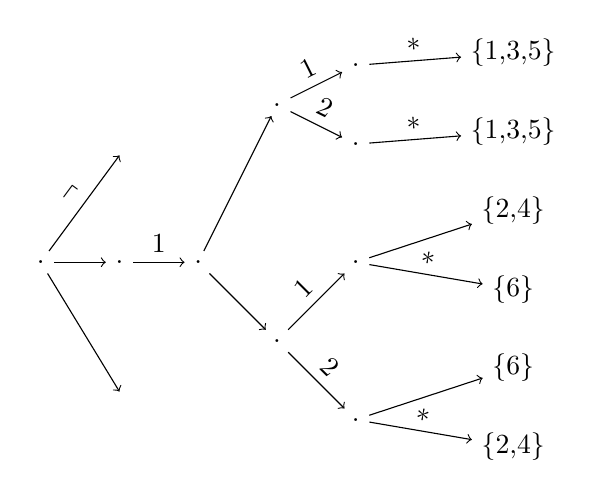
\begin{tikzpicture}[->,sloped,above]
	
	\node (root) at (0,2.5) {.};
	
	\node (h) at (1,2.5) {.};
	
	\node (h1) at (2,2.5) {.};
	
	\node (h1f) at (3,4.5) {.};
	\node (h1g) at (3,1.5) {.};
	
	\node (h1f1) at (4,5) {.};
	\node (h1f2) at (4,4) {.};
	\node (h1g1) at (4,2.5) {.};
	\node (h1g2) at (4,0.5) {.};
	
	\node (h1f1x) at (6,5) {\{1,3,5\}};
	\node (h1f2x) at (6,4) {\{1,3,5\}};
	\node (h1g1a) at (6,3) {\{2,4\}};
	\node (h1g1x) at (6,2) {\{6\}};
	\node (h1g2a) at (6,1) {\{6\}};
	\node (h1g2x) at (6,0) {\{2,4\}};
	
	\path (root) edge node {$\mP$} (h)
	(h) edge node {$1$} (h1)
	
	(h1)
	edge node {$\mf$} (h1f)
	edge node {$\mg$} (h1g)
	
	(h1f)
	edge node {$1$} (h1f1)
	edge node {$2$} (h1f2)
	
	(h1g)
	edge node {$1$} (h1g1)
	edge node {$2$} (h1g2)
	
	(h1f1)
	% edge node {$\ma$} (h1f1a)
	edge node {$*$} (h1f1x)
	
	(h1f2)
	%		edge node {$\ma$} (h1f2a)
	edge node {$*$} (h1f2x)
	
	
	(h1g1)
	edge node {$\ma$} (h1g1a)
	edge node {$*$} (h1g1x)
	
	(h1g2) 
	edge node {$\ma$} (h1g2a)
	edge node {$*$} (h1g2x)
	
	(root)
	edge node {$\lnot$} (1,4)
	edge node {$\mQ$} (1,1)
	;
	\end{tikzpicture}
\end{center}
$\lnot\mP(\mg(\mb,z)) \mapsto \{ \mP.1.\mg.1.{\mb}, \mP.1.\mg.2.{*} \} \mapsto \{6\} \cap \{2,4,6\}$}
% ==============================================================

% issues
%\frame{\input{../tikz/DiscriminationTree.tex}} % incomplete
% \frame{% !TeX spellcheck = en_US
% !TeX encoding = UTF-8

\begin{tikzpicture}[scale = 1, transform shape, draw=black, fill=black, thick, sloped]

	\draw[myarrow, ultra thick] (0,0) -- 
	node[pos=0, above] {$F$} 
	(2,0);
		
	% outer rectangle
	\draw[rounded corners=1.5mm,dotted] (0.5,3) rectangle (8.5,-3);
	% is F a theorem?
	\draw(1.9,2.7) node {Is $F$ a theorem?};
	
\pause
	% SLIDE Is S satisfiable?
	\node[colG] (S) at (1.1,-2.7) {\scriptsize$\lnot F \approx S$};
\pause
		\node (S) at (2.5,0) {$S$};
		

			% SLIDE 2
			\draw[thin,dashed,draw=colO] (2.5,0) ellipse (0.4 and 1.2); % S
			
			% inner rectangle
			\draw[very thick,draw=DarkGray]  (1.5,-2.25) rectangle (8,2.25); 
			% is S satisfaible?
			\draw (2.9,1.9) node {Is $S$ satisfiable?};
	
\pause
		% SLIDE unsatisfiable
		\draw[thin,dashed,draw=colO] (2.6,0) ellipse (0.6 and 1.44);  % S
		\draw[dashed, draw=colG, thick] decorate[decoration={snake}] {(1.4, 1) -- (8.2,0.6)};
		\draw[myarrow, draw=colHi, ultra thick] (6.5,1.8) -- 
			node[pos=0,below] {unsatisfiable}
			node[pos=0.85, above] {theorem} 
			(10,1.8) ;

\pause
		% SLIDE satisfiable
		\draw[thin,dashed,draw=colO] (2.8,0) ellipse (0.9 and 1.73);  % S
		\draw[dashed, draw=colG, thick]  decorate[decoration={snake}] { (1.4,-1)  --  (8.2,-0.6) };
		\draw[myarrow,draw=colLo, ultra thick] (7,-1.3) -- 
			node[pos=0, below] {satisfiable}
			node[pos=0.75, above] {not a theorem} (11,-1.3) ;
		 
\pause
		% SLIDE 5
		 \draw[thin,dashed,draw=colO] (3.2,0) ellipse (1.35 and 2.07); % S
		 	\draw[myarrow,draw=colNa, ultra thick] (7,0.15) -- 
		 	%	node[pos=0,above] {space out}
		 	node[pos=0,below] {time out}
		 	node[pos=0.85, above] {maybe} (10.5,0.15) ;

	\onslide<1->
\end{tikzpicture}}

\end{document}
